\chapter{Introduction}
% possible quotations: welcome humans. goodwill. and we have a plan.

Humanoid service robots of \company have a touchscreen on their torso.
Using a web application, users create content applications (e.g. buttons that trigger actions in the robot or a picture gallery) that can be displayed in the screens of the robots.
The software in the robots depends on \flash and needs to be reengineered with web technology.

This document is a stand alone presentation of the work done at \company , which belongs to a larger project: the Content Management System (codenamed \textit{Flango}).
\begin{figure}[htb]
    \centering
    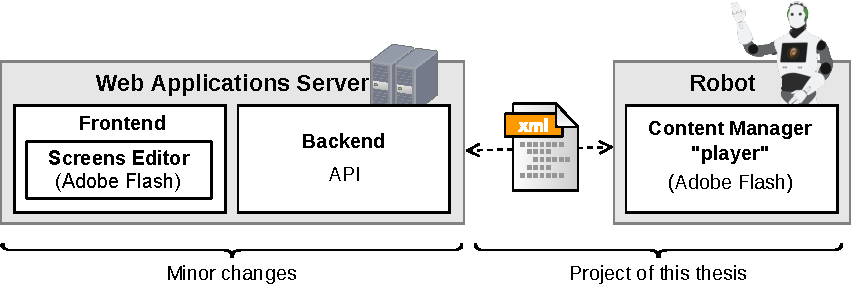
\includegraphics{figures/intro-system-overview.pdf}
    \caption{Overview of the Content Management System}
    \label{fig:intro-system-overview}
\end{figure}
More specifically, \textbf{this thesis deals with the reengineering of Flango \cm , the part of the system deployed \textbf{in the robot}} that displays content applications on the touchscreen of \reem{H} (\fref{fig:intro-system-overview}).
\textbf{It does not reengineer the rest of the system}, like the web application (that uses \flash as well) to generate content applications, although there might be minor changes to adapt their interfaces to the new technology.

It is desired not only to develop a practical solution but also to guarantee that the final output of the Flango \cm is the same that the old system generates.

This thesis is eminently a practical work, although the theoretical background has been extensively explored. 
Using web technology in a component of the robot is a novelty in the company. 
It is done to develop a sustainable product based on open standards (as opposed to the current implementation with \flash) that can be extended and reused for other robotic products that might be designed in the future.

\section{\company}
\company is a company based in Barcelona dedicated to R\&D of humanoid robots and robotic components. 
An international team of mostly mechanical, electronics and software engineers pushes forward the research on different fields, like speech recognition and generation, computer vision, walking, grasping, machine learning and navigation amongst others.
The company has developed 6 humanoid robots until 2013: \reem{A}, \reem{B}, \reem{H1}, H2 and H3, and \reem{C}.
This project targets \reem{H2} and H3, service robots with wheels and touchscreen.

\subsection*{Reem H2 and H3}
\reem{H2} (\fref{fig:reemh2}) and H3 (\fref{fig:reemh3}) are humanoid service robots featuring a screen on their torso.
They have an autonomous navigation system, speech recognition and voice synthesiser, they can find their way in different settings and help or entertain people in a friendly way.
They are intended for use in public places such as hotels, malls, airports or museums.

\begin{figure}
   \centering
   \begin{subfigure}[b]{0.4\linewidth}
       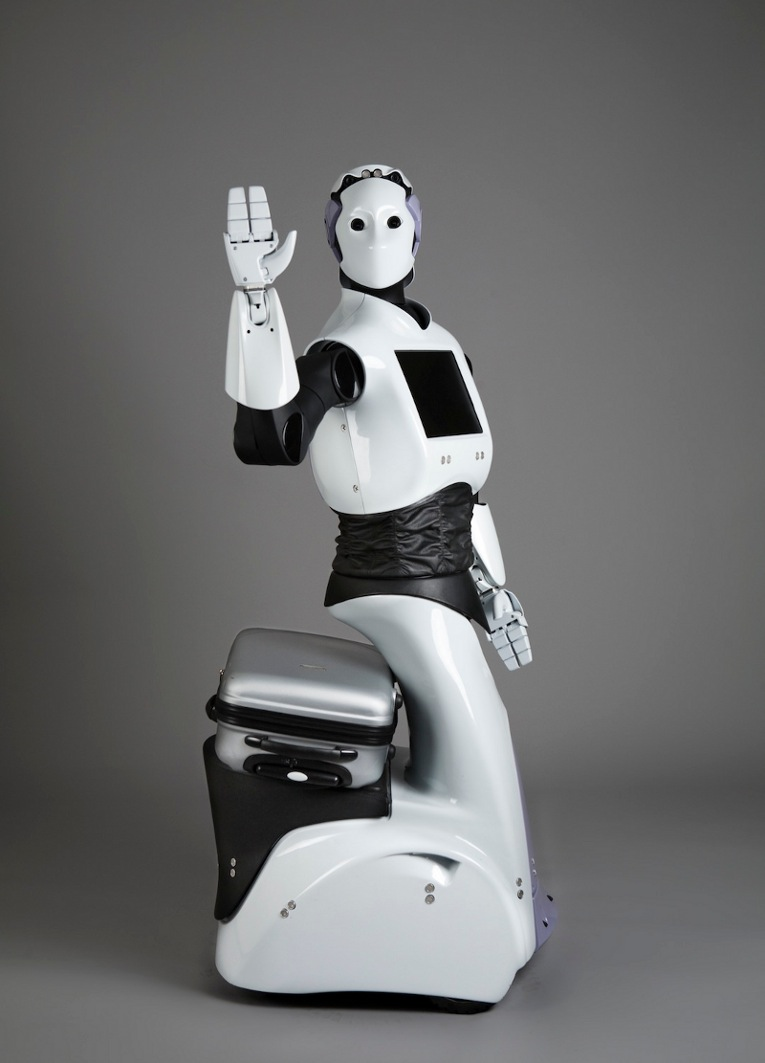
\includegraphics{figures/reemh2}
       \caption{\reem{H2}}
       \label{fig:reemh2}
    \end{subfigure}
    \begin{subfigure}[b]{0.4\linewidth}
           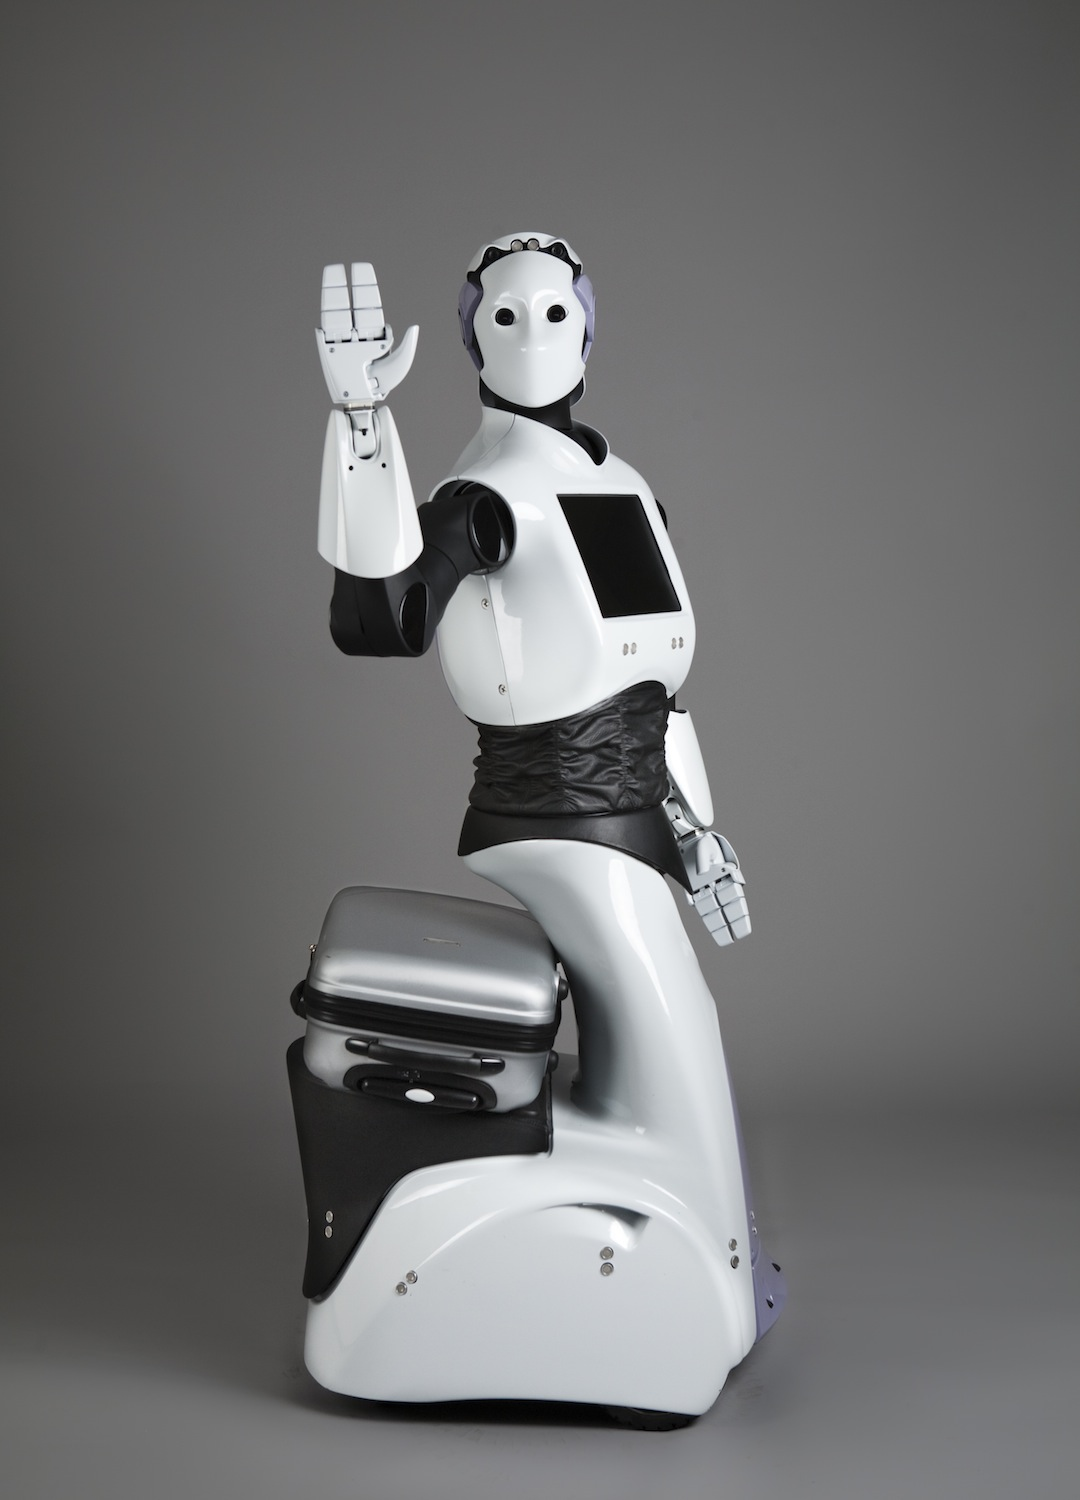
\includegraphics{figures/reemh3}
           \caption{\reem{H3}}
           \label{fig:reemh3}
    \end{subfigure}
    \caption{\reem{H} Series}
    \label{fig:reemseries}
\end{figure}
\FloatBarrier
\begin{table}
    \centering
    \begin{tabularx}{\linewidth}{| X | X |}
    \hline
    Weight & 90 Kg\\ \hline
    Height & 1.70 m \\ \hline
    Battery life & 8 h \\ \hline
    Degrees of freedom & 22 \\ \hline
    Payload & 30 Kg (mobile base), 3 Kg/arm\\ \hline
    Speed & 4 Km/h\\ \hline
    Computer & Core 2 Duo + Atom\\ \hline
    Sensors & Microphone, stereo-camera, laser, ultrasounds, accelerometers and gyroscopes\\
    \hline
    \end{tabularx}
    \caption{Reem H2 and H3}
    \label{tab:rh2}
\end{table}
\FloatBarrier
\section{The Current System}
The \reem{H} series have a multi-modal interface: besides speech or joystick manual control, humans can use a touch screen to command the robot or obtain information.
\reem{H} can display multimedia contents like videos, facts about a company, robot features, language settings, etc.

The Contents Management System comprises \emph{\flangofe} and \emph{\flangobe} (both in Basestation), and \emph{Flango \cm} (in the robot) (see \fref{fig:intro-system-overview}).
The Basestation is an application server that hosts Flango, a \ac{RIA} to manage contents and robots made with Django, a widely used framework for Python. 
Clients can create content applications  with the \flangofe (\se), a tool built with \flash .
When content applications are ready, clients can associate $1$ application with $n$ robots to display it in the touch screen.

\lstinputlisting[label=example-screen-xml,language=XML, caption={Example Screen XML}, breaklines=true]{src/example-screen.xml}

The elements of a content application (screens and entities) have an \ac{XML} representation (listing \ref{example-screen-xml}), an approach similar to popular projects (e.g. Android, NetBeans) and even, in a sense, all \acp{RIA} made with \ac{HTML}.

The Flango \cm interprets the \ac{XML} and displays the result on the screen (\fref{fig:xml-flango-view}).

A content application is essentially a set of screens, navigation, multimedia contents, and entities. 
The latter are domain objects that can be instantiated and represented in a view. 
This way a user can create an application that shows information about the company, include buttons to provide an easy way to give commands to the robot (e.g. "follow me", "shake hands"), display videos and picture galleries, etc.
All of these components are localisable:  
They can be resized, repositioned, repainted... depending on the active language.
Using other tools, clients can also associate sentences to screens and the text-to-speech system reads them aloud.

\begin{figure}[htb]
    \centering
    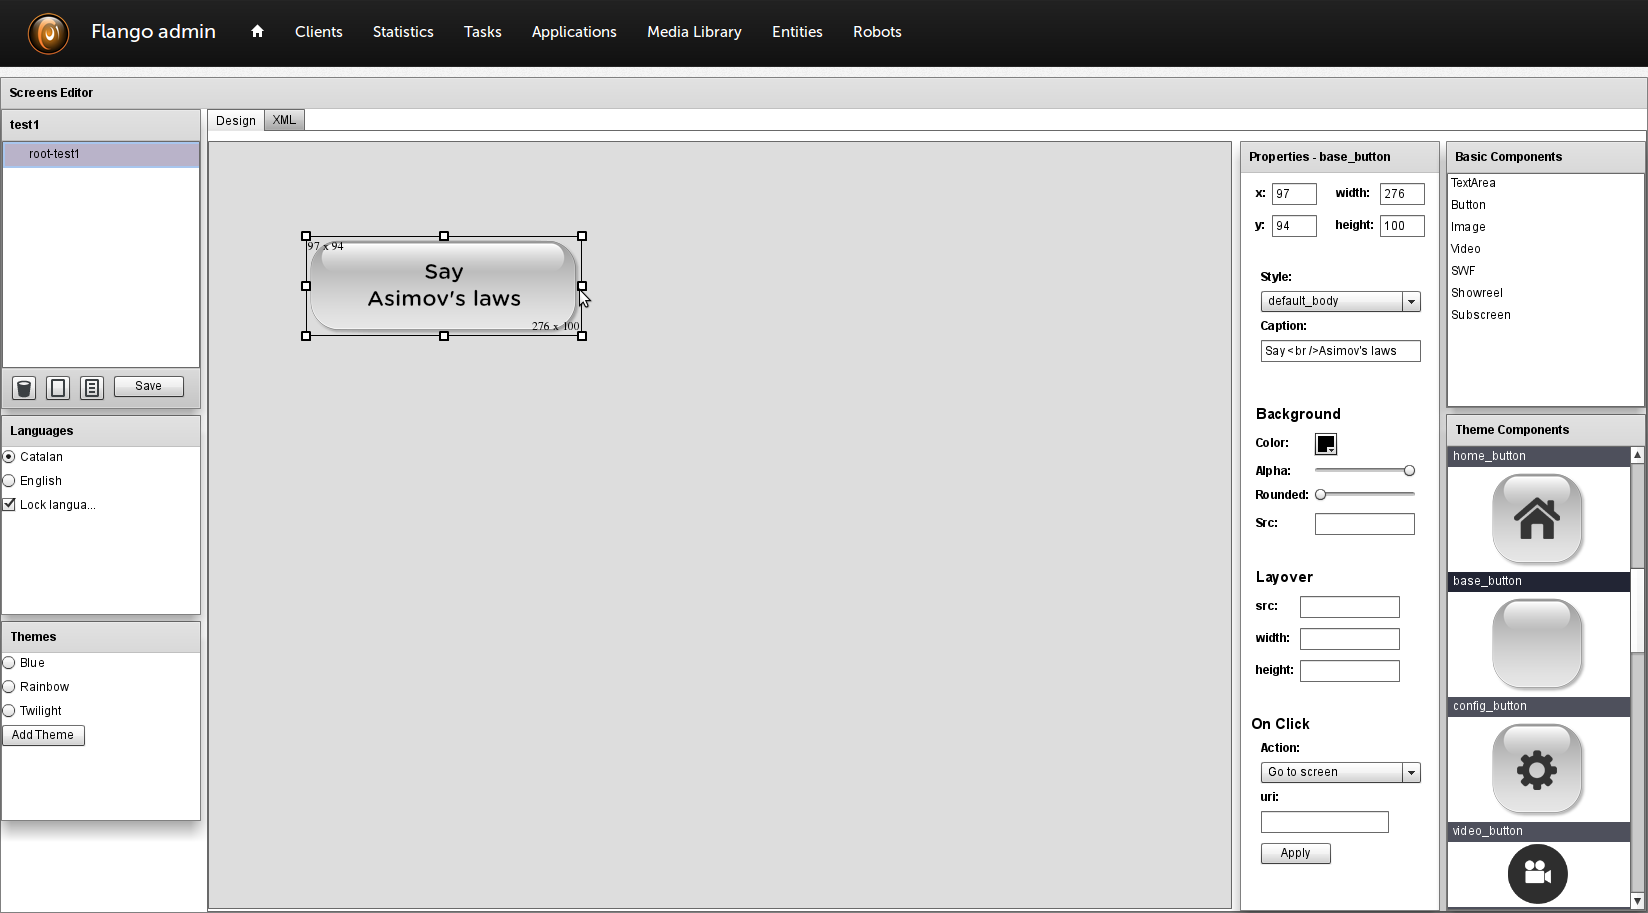
\includegraphics[width=\textwidth]{figures/screens-editor}
    \caption{\se , a \flash application in Flango}
    \label{fig:screens-editor}
\end{figure}

\reem{H} robots have a built-in software to display the content applications, the Flango \cm , which is also made with \flash .
Initially, this software has no \ac{GUI} or direct interaction with a person.
It transforms \ac{XML} files into a \ac{UI} (\fref{fig:xml-flango-view}) and, finally, displays the screens and manages the user interaction (e.g. clicks on a button).

\begin{figure}[htb]
    \centering
    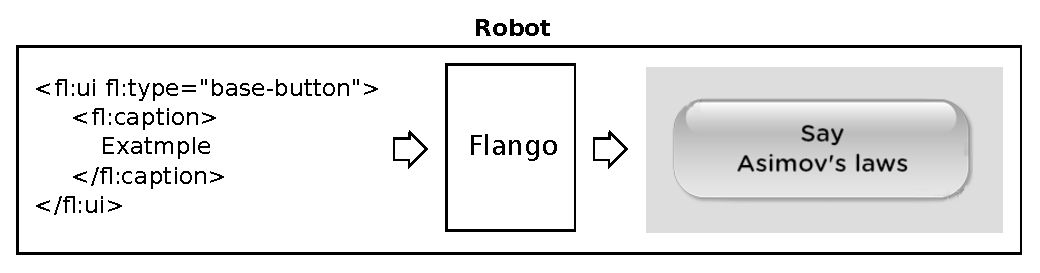
\includegraphics[width=\textwidth]{figures/xml-flango-screenshot}
    \caption{Transformation of \acs{XML} into a \acs{GUI}}
    \label{fig:xml-flango-view}
\end{figure}

\textbf{This thesis documents the project of reengineering the \cm , in the robot, with web technology instead of \flash , namely \acs{HTML5}, \acs{CSS3} and \acf{JS}}.

\section{The New System}
The \ac{WWW} was born as a document viewing platform and has evolved gradually into an application platform. 
First the web consisted of simple pages that contained structured text and some images. 
Navigation was done using simple links between pages. 
In a second phase, web sites became interactive: 
it was the time of animated graphics, browser plug-ins and JavaScript. 
More recently web sites have adopted features from traditional desktop software in \acp{RIA} \cite{Anttonen:2011}.

For a decade, the \flash player plug-in has provided a platform to enable rich and interactive content in browsers.
However, Adobe has made the updates exclusive to the Google Chrome\textsuperscript{\textcopyright}\xspace browser \cite{FlashRoadmap}. 
The browser in the robot application, QtWebBrowser, uses this plug-in but will not receive updates from Adobe. \company ' systems need to adapt to this new setting. 
There are two solutions:
\begin{itemize}
	\item Use Google Chrome instead of QtWebKit
	\item Use modern web technologies, either in QtWebKit or in another browser
\end{itemize}

The solution is rethinking the application to be a part of the robot's system and implement it with modern web technology.
There is a number of technologies that could be used, but the Web allows the product to be easily portable, very extensible, open to many developers and sustainable as it does not depend on a single company.
\ac{HTML5} is perhaps the best known forthcoming standard in the Web and is typically combined with JavaScript and \ac{CSS3}. 
It has become such a popular combination that major browser vendors provide support for the latest drafts of the \ac{W3C}, like the audio \ac{API} for \ac{HTML5} or the video support.
A big number of frameworks with JavaScript have appeared not only client-side (e.g. BackBone, jQuery, Ext JS, Google Web Toolkit, Yahoo User Interface Library...), but even server-side (e.g. NodeJS).
Moreover, new \ac{HTML5} capabilities and \acp{API} are an opportunity to add features to this project.

The project of this thesis uses Google Angular\textsuperscript{\textcopyright}, a \ac{MVC} framework that lets developers \emph{teach the browser new syntax}. 
Thus, \ac{XML} files created with the \se can be interpreted natively in a browser. 
This has some advantages over \flash \cite{Jobs:ThoughtsOnFlash}:
\begin{itemize}
    \item No use of third-party plug-ins
    \item Openness
    \item Reliability, security and performance
    \item Keeps power consumption lower (e.g. using the GPU to decode video or apply transformations and smooth transitions to elements on the screen)
    \item Touch-enabled: the new screen of Reem H3 is multi-touch. To enable gestures, heavy rewriting of the current Flash application is required.
\end{itemize}


\section{Goals}
This thesis is part of the specialisation of \emph{Software Engineering and Information Systems}. 
The goal is to reengineer the Flango \cm with web technology.
More specifically, the author has to gather the requirements from an existing system, plan in terms of scope, time and cost, make the system specifications, design and implement it using modern web technologies, use quality assurance tools and deploy it successfully in a \reem{H3} robot.

Regarding the project, the goals are:
\begin{itemize}
	\item Reengineer the current system with web technology
	\item Develop a testing strategy to make it robust
	\item Make it compatible with non-reengineered parts of the system
\end{itemize}


\section{Organisation of This Document}
This document describes the system developed at \company to display the  content applications created with the \se on the \reem{H} series.
It does not cover other software on the robots or in Basestation.

This document describes the project as follows:
\begin{description}
\item[Related Work] Provides a general overview of topics surrounding those of this thesis, enabling for a deeper understanding of the material at hand.
It starts with a description of the reengineering process, followed by a section about web technology and, finally, a description of the methodology of the project -- \ac{TDD}.

\item[Project Management] Contains information about the project from the point of view of management. 
Detailing on schedule, budget and risk analysis. Contains an assessment of the execution.

\item[Requirements] States the functional and non-functional minimum requirements, the constraints and weights the use of off-the-shelf solutions.

\item[Specification] Defines what the application does in the context of a reengineering process. 
It deals with the first three steps: a software inventory, documentation restructuring and a description of the current system (with special attention to context, interoperability and interaction).
Contains the specification of the new system: a conceptual model, use cases and the behaviour model, with sequence diagrams and contracts of system operations. 

\item[Design] Describes the internal design of the software in the context of a reengineering process. 
It contains the last three steps: code restructuring, data restructuring and forward engineering.
Detailing about the system architecture and the context and the patterns used.
Contains a static view (class and packages diagram), a dynamic view (sequence diagrams) with examples of the most relevant operations and a physical view (deployment diagrams).

\item[Implementation] Holds technical details about the environment, the set-up, the integration in the robot and a larger system and meaningful examples of the technology used. 
Emphasises the implementation of the patterns described in previous chapters.

\item[Testing] Highlights the strategy to implement tests and the integration in the robot system.

\item[Conclusion] Presents the conclusions from technical, academic and personal point of view. 
Includes challenges faced during developments and future work. FIXME

\item[Appendix A] Lists UI Components of the old system.

\item[Appendix B] Lists unit tests that define the behaviour of most components of this system.

\end{description}